
\section{State of the art}

\subsection{Quaternion representation}

A quaternion is a four-dimensional vector, defined as 

\begin{center}
$ \mathbi{q} = \begin{pmatrix} \textbf{q} \\ q_w \end{pmatrix} $ with $ \textbf{q} =  ( q_x, q_y, q_z)^T $. 
\end{center}

For attitude representation, the quaternion must satisfies a single constraint given by  $|| \mathbi{q}  || = 1$.

Then, the attitude matrix $R \in SO(3) $ related to the quaternion $\mathbi{q}$ is given by :
\vspace{-0.15cm}
\begin{equation}
R(\mathbi{q}) = (q_w^2 - |\textbf{q}|^2)I + 2 \textbf{q}\textbf{q}^T - 2q_w[\textbf{q} \times]
\label{quat_to_rot}
\end{equation}

Where $SO(3)$ is the special orthogonal group defined by:
\vspace{-0.15cm}
$$SO(3) = \{ R \in \mathbb{R}^{ 3 \times 3} | RR^T = R^TR = I, det(R) = 1 \}$$

And $[\textbf{v} \times] \in \mathbb{R}^{3\times 3}$ is the skew-symetric matrix of the vector $\textbf{v}$ such as.

\begin{equation}
[\textbf{v} \times] = \begin{pmatrix} 0 & v_z & -v_y \\ -v_z & 0 & v_x \\ v_y & -v_x & 0 \end{pmatrix} 
\label{skewsymmat}
\end{equation}


\subsection{Most Common Fusion Methods}


\subsubsection{Kalman Filter}

Introduced in 1960 by Kalman \cite{kalman_new_1960}, the Kalman filter is an algorithm that uses a series of measurements observed over time, containing noise, in order to estimate unknown variables (state vector). Based on a model it is possible to obtain a more robust estimation of the state vector. Consider the following linear system, described by the difference equation and the observation model with additive noise:


\begin{equation}
\left\{ \begin{array}{l}
\textbf{x}_{k+1} = F_{k}\textbf{x}_{k}+B_{k}\textbf{u}_{k}+G_{k}\textbf{v}_{k}\\
\textbf{z}_{k} = H_{k}\textbf{x}_{k}+D_{k}\textbf{w}_{k}
\end{array} \right.
\label{linear_system}
\end{equation}

with,

\begin{center}
\begin{tabular}{rl}
$\textbf{x}_{k} $ &State vector at time $k$\\
$\textbf{z}_{k} $ &Measurement vector at time $k$\\
$\textbf{u}_{k} $ & Input vector (e.i.: from sensor) at time $k$ \\
$\textbf{v}_{k} $ & State noise vector disturbing the system\\
$\textbf{w}_{k} $ & Observation noise disturbing the measurement\\
\end{tabular}
\end{center}

\vspace{0.2cm}


A brief presentation of the algorithm is provided here,  see \cite{terejanu2013discrete} for more details. The algorithm has 3 important steps :\\

\begin{itemize}
\item The first step is the \textbf{prediction} of state $\textbf{x}^-_{k+1}$ at time $k+1$ and covariance $P^-_{k+1}$ is given by :

\begin{equation}
\left\{ \begin{array}{cl}
\textbf{x}^-_{k+1} = & F_{k}\textbf{x}^+_{k} + B_{k}\textbf{u}_{k} \\
P^-_{k+1} = & F_{k}P^+_{k}F^T_{k}+G_{k}Q_{k}G^T_{k}
\end{array}
\right.
\end{equation}

\item The \textbf{innovation} is the difference between predicted measurement and real measurement. It measure up the deviation used by the Kalman gain.
\begin{equation}
\left\{ \begin{array}{cl}
\boldsymbol\nu_{k+1} = & \textbf{z}_{k+1}-H_{k+1}\textbf{x}^-_{k+1} \\
\mathcal{S} = & R_{k+1} +H_{k+1}P^-_{k+1}H^T_{k+1}
\end{array}
\right.
\end{equation}

\item And finally, An \textbf{update} is processed to correct the estimate state $\textbf{x}^+_{k+1} $ and his covariance $P^+_{k+1}$ with the innovation.

\begin{equation}
\left\{ \begin{array}{cl}
\textbf{x}^+_{k+1} = & \textbf{x}^-_{k+1} + \mathcal{K}_{k+1}\boldsymbol\nu_{k+1} \\
P^+_{k+1} = &P^-_{k+1} - \mathcal{K}_{k+1}S_{k+1}\mathcal{K}^T_{k+1}
\end{array}
\right.
\end{equation}

\end{itemize}

Where $\mathcal{K}_{k+1}$ is the Kalman gain  representing relative importance of innovation  $\nu_{k+1}$. 

\begin{equation}
\mathcal{K}_{k+1}=P^-_{k+1}H^T_{k+1}\mathcal{S}^{-1}
\end{equation}

The Kalman filter provides an optimal estimation for linear systems. Nevertheless, most of studied dynamical systems are nonlinear (attitude estimation, pendula, ... ). Thus, extended Kalman Filter approach  was proposed for nonlinear systems \cite{larson1967application, larson1967precomputation,terejanu2008extended}. 

Here, we have chosen to use quaternions for the attitude representation because of its singular-free specificity. But special care must be taken when designing a quaternion based extended Kalman filter. Because of the constraint on the quaternions, the covariance matrix $P$ can be singular \cite{vik2009integrated} which is problematic for the numerical stability. There exist several methods to deal with this issue. Multiplicative Extended Kalman Filter (MEKF)\cite{markley2003attitude} and the Additive Extended Kalman Filter (AEKF) \cite{bar1991quaternion} are designed to tackle this problem.The difference between AEKF and MEKF is discussed in \cite{markley_multiplicative_2004}. For the library, we choose to implement MEKF.

On the other hand, the Unscented Kalman Filter method was proposed by Julier and Uhlmann \cite{julier_new_1995} in 1995 . It belongs to a class of filters called Sigma-Point Kalman Filters. Instead of using the Taylor series expension, UKF use an unscented transformation \cite{uhlmann1995dynamic} to approximate the nonlinear projection of mean and covariance of a probability distribution. For the library, we choose to implement the filter proposed by Crassidis et al. called UnScented QUaternion Estimator (USQUE) \cite{crassidis_unscented_2003}, based on UKF. They used the same representation as MEKF.

\subsubsection{Nonlinear Observer}

The theory of the state observer was first introduced by Kalman and Bucy for a linear system in a stochastic environment. Then Luenberger \cite{david1971introduction} made a general theory of observers for deterministic linear systems, introducing the notions of observer and reduced minimum observer \cite{primbs1996survey}. Mahony et al. \cite{mahony_nonlinear_2008} have proposed an nonlinear observer called Constant Gain Observer (CGO), termed the explicit complementary filter, that provides attitude estimates as well as gyro bias estimates. 

One problem of Kalman Filters is to find the initial values in the covariance (matrix $Q$) because it is difficult to relate it to real physical quantities. The covariance matrix is not involve in nonlinear observer theory. This is one of the reasons there has been an increasing interest for nonlinear observer design the last decades. Another reason is their low computational need.

\subsubsection{Methods Based on Solutions of the Wahba's Problem}

The attitude determination problem for vector observation was first formulated as a least squares estimation problem by Wahba \cite{wahba_least_1965} in 1965 :\\


Given the two sets of $n$ vectors $\{ \textbf{r}_{1},...,\textbf{r}_{n} \}$ and $\{ \textbf{b}_{1},...,\textbf{b}_{n} \}$, $n \geqslant 2 $, where each pair $(\textbf{r}_{i},\textbf{b}_{i})$ corresponds to a generalised vector, $\textbf{x}_{i}$, find the proper orthogonal matrix, $A$, which bring the first into the best least squares coincidence with the second. That is, find $A \in SO(3)$ which minimises the function $J$ defined as:

\begin{equation}
J(A) = \frac{1}{2} \sum_{i=1}^n a_i||b_i-Ar_i||^2
\label{Wahba_loss_function}
\end{equation}

The equation (\ref{Wahba_loss_function}) can be written with a quaternion representation which gives:

\begin{equation}
J(\mathbi{q}) = \frac{1}{2} \sum_{i=1}^n a_i||b_i-R(\mathbi{q})r_i||^2
\label{QUEST}
\end{equation}

The matrix $R(\mathbi{q})$, is the rotation matrix that corresponds to the quaternion $\mathbi{q}$ (equation \ref{quat_to_rot}). The QUEST algorithm are conducted in the following manner. Let

\begin{equation}
B = \sum_{i=1}^N a_i\textbf{b}_i \textbf{r}_i^T
\end{equation}

Then, we can rewrite the equation (\ref{QUEST}) as follow

\begin{equation}
J(\mathbi{q}) = \frac{1}{2} \sum_{i=1}^n a_i  - tr(R(\mathbi{q})B^T)
\label{QUEST_bis}
\end{equation}

Due to the fact that the representation of the attitude matrix is a homogenous quadratic function of $\mathbi{q}$, we can say that

\begin{equation}
tr(R(\mathbi{q})B^T) = \mathbi{q}^TK\mathbi{q}
\label{QUEST_ter}
\end{equation}

where $K$ is the symmetric traceless matrix such as

\begin{equation}
K = \begin{pmatrix} S-tr(B)I_3 & \textbf{z} \\ \textbf{z}^T & tr(B)
\end{pmatrix}
\end{equation}

with

\begin{equation}
\left\{\begin{array}{l}
S = B + B^T\\
\textbf{z} = \sum_ia_i\textbf{b}_i\times\textbf{r}_i
 \end{array}
\right.
\end{equation}


The minimisation problem from Equation (\ref{QUEST_bis}) is now a maximisation problem. thus, the solution $\mathbi{q}_{opt}$ is the eingen vector correspond to the largest eigen value of $K$ \cite{markley1999estimate}. The main problem of QUEST is that it does not take into account of all the previous observations performed since the beginning. A recursive QUEST algorithm (REQUEST) proposed by Bar-Itzhack manages this problem.  Contrary to other methods, the QUEST algorithms do not estimate the gyroscope bias. Which can make it less robust in some cases.

There are also other methods based on Wahba's problem like the Davenport's q-method \cite{weighted1971nasa} proposed in 1971 considered more robust than QUEST. Or the method ESOQ proposed by Mortari \cite{mortari1997esoq}  in 1997. However, for this library, we limit our investigation to REQUEST.\\



\subsubsection{Particle Filtering Method}

Particle filtering method is based on Monte-Carlo method\cite{metropolis1949monte}. The main idea is to use a large number of samples called particles to estimate a nonlinear function \cite{chen_bayesian_2003} and \cite{terejanu2009tutorial}. The set of $N$ particle with associated weight at time $k$ are denoted by $\{\textbf{x}^{(i)}_{k},w^{(i)}_{k}\}$. Initially, the particle are drawn from a proposal distribution. The PF is divided into three step, prediction, update, resampling, that constitute a filter cycle:

\begin{itemize}
\item Prediction
\end{itemize}

The first step is to propagate all particles $\{\textbf{x}^{(i)}_{k},w^{(i)}_{k}\}$ to $\{\textbf{x}^{(i)}_{k+1},w^{(i)}_{k+1}\}$ with the nonlinear function $f$ while the weight remain unchanged : 

\begin{equation}
\textbf{x}^{(i)}_{k+1} = f(\textbf{x}^{(i)}_{k},\textbf{u}_{k}) + \textbf{w}_{k}^{(i)}\\
\end{equation}

where $N$ sample $\textbf{w}_{k}^{(i)}$ of the process noise (supposed gaussian in our case) are drawn.

\begin{itemize}
\item Update/Correction
\end{itemize}

At the update step, the weights associated with each particle is updated based on the likelihood function $p( \textbf{z}_{k+1}| \textbf{x}_{k+1}^{(i)})$.
\begin{equation}
\left\{ 
\begin{array}{l}
w_{k+1}^{(i)} = w_{k}^{(i)} p( \textbf{z}_{k+1}| \textbf{x}_{k+1}^{(i)})\\
\tilde{w}_{k+1}^{(i)} = \frac{w_{k+1}^{(i)}}{\sum_iw_{k+1}^{(i)}}
\end{array}
\right.
\end{equation}

The weight are normalised such as we have $\sum_i\tilde{w}_{k+1}^{(i)}=1$. To finish, the mean is computed with the following equation:

\begin{equation}
 \textbf{x}_{k+1}^+ = \sum_{i=1}^N\tilde{w}_{k+1}^{(i)} \textbf{x}_{k+1}^{(i)}
 \end{equation}



\begin{itemize}
\item Resampling/Regularisation
\end{itemize}

A common problem with PF is the degeneracy phenomenon. After some iterations, more and more particles will have a weak weight, which make them negligible and useless.  To overcome this problem, a regularisation step called resampling is processed. It is not needed to perform PF but it allows to maintain a good performance relative to degeneracy problem. The idea of resampling is to eliminate particles having feeble weight and focus on strong weight particles. In order to measure degeneracy, the number of effective samples $N_{eff}$ is computed (equation \ref{N_eff}). If  $N_{eff}$ is lower than a threshold, the resampling step is processed.

\begin{equation}
 N_{eff} = \sum_{i=1}^N\frac{1}{(\tilde{w}_k^{(i)})^2}
 \label{N_eff}
 \end{equation}


The choice of the threshold is important. Indeed, a high threshold gives $N_{eff} \approx N$, but that does not mean necessarily we have a lot of efficient particles. On the contrary, it means that most of the particle are identical making large computations unnecessary. Moreover, with a low threshold, many particles are neglected making computations less efficient. In general, the threshold is fixed at  $\frac{N}{2}$ or $\frac{N}{3}$. There are several types of resampling, a comparison is made in \cite{douc2005comparison}. We took the resampling algorithm described in \cite{arulampalam2002tutorial} because it is the most commun. Cheng, Yang and Crassidis have propose an attitute estimation with a particle filter method \cite{cheng_particle_2010}. We have also considered the revisited algorithm of Cheng \cite{chang_particle_2014} based on bootstrap filter\cite{gordon1993novel}. We have chosen to implement this one because they use the same approach as USQUE \cite{crassidis_unscented_2003} and MEKF\cite{markley2003attitude}. We decided to explore the performance of this three algorithms with the same model. The particle filter provides an estimate of the nonlinear system without assuming that the noise is Gaussian. So it is more robust to any situation, which makes it more performant in the context of a real applications. But an important computation time is required and that is a limitation for a real-time application.



\section{Performance Evaluation}

\subsection{Score definition}
We have access through our designed ground truth (simulated or from computer vision technics) to the true attitude $\mathbi{q}^{real}_k$ at time $k$ of the reference frame $\{c\}$ related to $\{a\}$.
By computation, each method returns an estimate attitude $\mathbi{q}^{est}_k$ at time $k$ (see figure \ref{test_method}). 

\begin{equation}
 \delta \mathbi{q}_k = \mathbi{q}^{real}_k \otimes (\mathbi{q}^{est}_k)^{-1} =  \begin{pmatrix}  \delta \textbf{q}_{k} \\ \delta q_{w_k}  \end{pmatrix}
\end{equation}

The error-MRP vector related to $ \delta \mathbi{q}_k$ is given by

\begin{equation}
 \delta \textbf{p}_k  = 4[\frac{\delta \textbf{q}_{k}  }{(1+\delta q_{w_k})}]
\end{equation}


Thus, we can calculate the attitude error given by the root mean square (RMS) of $\delta \textbf{p}_k$:

\begin{equation}
\epsilon_k  = RMS (\delta \textbf{p}_k) = \sqrt{\frac{1}{3}( \delta p_{k_x}^2 +\delta p_{k_y}^2+\delta p_{k_z}^2)  }
\label{error_definition}
\end{equation}

The mean of the error is given by :

\begin{equation}
\bar{\epsilon}  = \frac{1}{n}\sum_{i=1}^n \epsilon_i \\
\label{mean_var_error_def}
\end{equation}

With $n$ the number of data at our disposal. We use this information (mean error) for our performance study. 

\begin{figure}[!h]
\centering
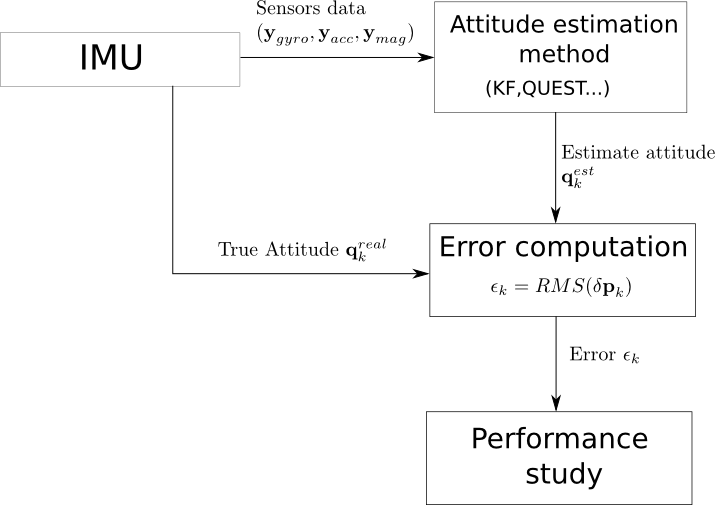
\includegraphics[scale=0.40]{images/test_method.png}
\caption{Algorithm designed to compute attitude estimation methods' performances}
\label{test_method}
\end{figure}


To differentiate the methods, we assigned  some ''scores'' in order to highlight the behaviour of these methods in different configurations. We defined these ''scores'' as:

\begin{align}
s_1 = \bar{\epsilon}\\
s_2 = \frac{1}{\bar{\epsilon} \times \bar{\tau}}
\label{score}
\end{align}

With $\bar{\epsilon}$ average attitude error (voir \ref{error_definition}) et $\bar{\tau}$ the average computation time. \\

\subsection{Simulated environment}

We  modelled our inertial sensors based on the Fossen's model \cite{fossen_handbook_2011}. The noise generated here is Gaussian. In this study, sensor bias are not considerate as constant. We proceed 30 consecutive simulations in order to get valid results. We've used  specification described in table \ref{spec_imu}. 

\begin{table}[!h]
\begin{tabular}{|c|c|c|}
\hline
Sensor & Bias instability  & Measurement noise\rule[-2pt]{0pt}{10pt} \\
\hline
\hline
 Gyroscope & $0.316\times 10^{-4} $  $\mu$rad.s$^{-\frac{3}{2}}$ & $ 0.316$  $\mu$rad.s$^{-\frac{1}{2}}$ \rule[-1.5pt]{0pt}{13pt}\\
 \hline
Magnetometer & $0.0023$ mGauss$/\sqrt{Hz}$ & 0.05 mGauss  \rule[-1.5pt]{0pt}{13pt}\\
 \hline
Accelerometer &  $0.002$ m.s$^{-2}/\sqrt{Hz} $ & 0.02 m.s$^{-2}$ \rule[-1.5pt]{0pt}{13pt}\\
 \hline
\end{tabular}
\caption{Calibrated IMU data performance specification, Gyrometer, Accelerometer, Magnetometer}
\label{spec_imu}
\end{table}



All simulations started with an initial attitude error $\delta\mathbi{q}_0$ randomly generated through normal distribution $\mathcal{N}(20,50^2)$. The results of score $s_1$ (resp $s_2$) are shown in figure \ref{histo_s1_add} (resp \ref{histo_s2_add}). Mean computation times of all methods required for one iteration is given in table (\ref{mean_time}).

\begin{table}[!h]
\centering
\begin{tabular}{|c|c|}
\hline
Method & Mean Computation time \\
\hline
\hline
CGO & $7.88 \times 10^{-6} s$\rule[-2pt]{0pt}{10pt}\\
 \hline
MEKF & $1.12\times 10^{-4} s$\rule[-2pt]{0pt}{10pt}\\
 \hline
 USQUE & $1.63\times 10^{-4} s $\rule[-2pt]{0pt}{10pt}\\
 \hline
PF & $4.5\times 10^{-2} s$\rule[-2pt]{0pt}{10pt}\\
 \hline
REQUEST& $1.91\times 10^{-4} s$ \rule[-2pt]{0pt}{10pt} \\
 \hline
\end{tabular}
\caption{Mean computation times for one iteration}
\label{mean_time}
\end{table}



\begin{figure}[!h]
\begin{subfigure}{.5\textwidth}
\centering
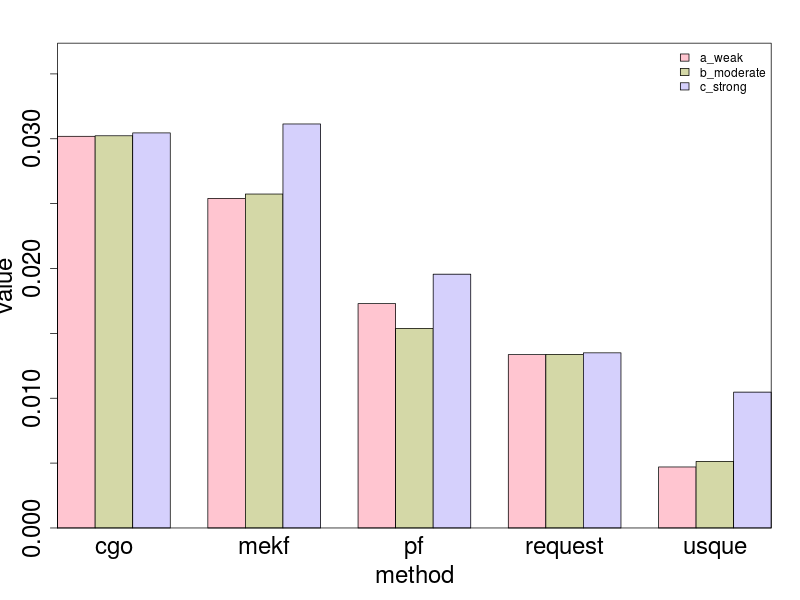
\includegraphics[scale=0.28]{images/histo_s1_add.png}
\caption{Scores $s_1$}
\label{histo_s1_add}
\end{subfigure}

\begin{subfigure}{.5\textwidth}
\centering
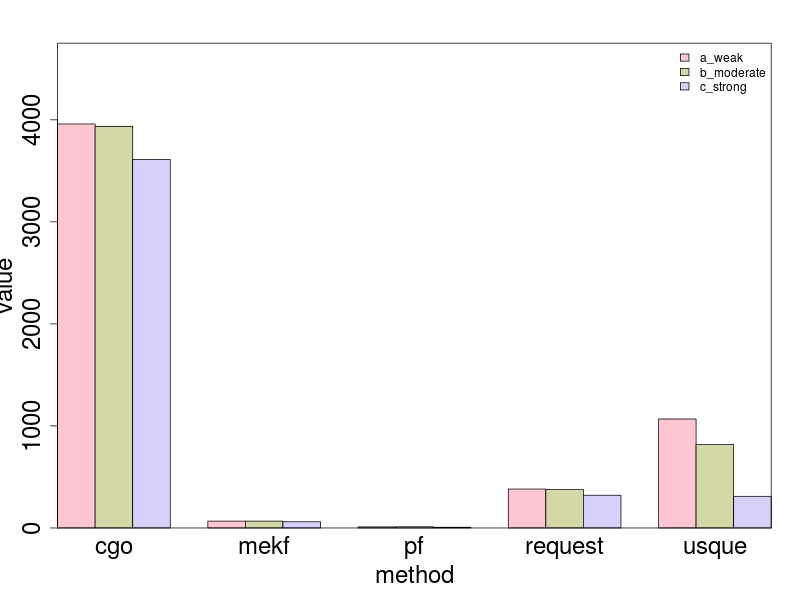
\includegraphics[scale=0.28]{images/histo_s2_add.png}
\caption{Scores $s_2$ }
\label{histo_s2_add}
\end{subfigure}
\caption{Scores $s_1$ (accuracy) and $s_2$ (accuracy and computation time ratio) of methods where noise is AWGN with 3 strength (weak, moderate, strong)}
\end{figure}

\subsection{Experimental validation}

We have designed a system that can be easily repeatable in laboratory. We used a smartphone as our IMU and a calibrated webcam (see figure \ref{situation_validation} ). With this system, we have defined our ground-truth as follows. A marker is stuck on the smartphone and we calculate an estimate of the attitude of the marker (which represents the smartphone) relative to the reference frame of the webcam $\{w\}$. We used the library \texttt{ArUco}  as optical feedback. At the same time, we get the data from the IMU of the smartphone to proceed the attitude estimation with our different algorithms.


\begin{figure}
\centering
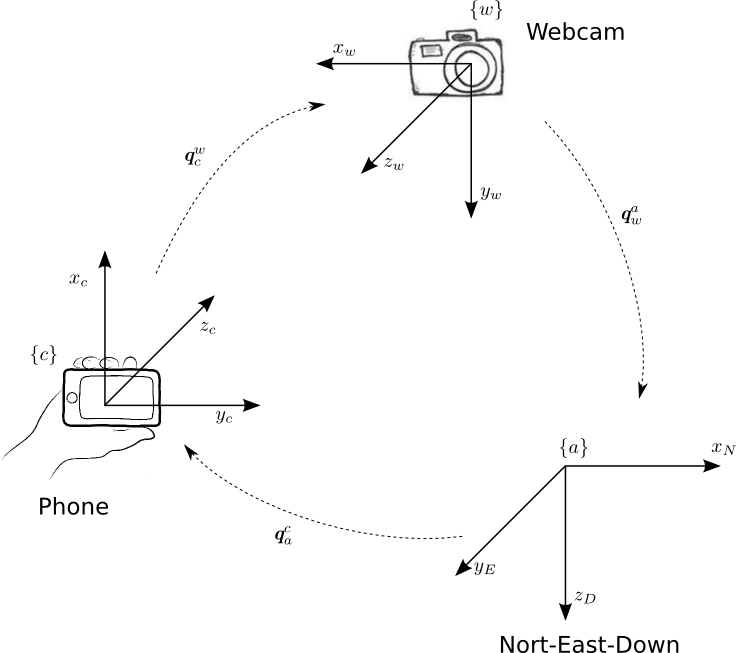
\includegraphics[scale=0.35]{images/situation_validation.png}
\caption{Representation of different reference frame used in this experiment. Here, only $ \text{\mathbi{q}}_w^a $  does not change.}
\label{situation_validation}
\end{figure}



At time $t = 0$, the camera and the smartphone has been set such as attitude quaternions $\mathbi{q}^a_w$, $\mathbi{q}^c_a$ et $\mathbi{q}^w_c$ are approximatively known. The camera being fixed, $\mathbi{q}^a_w $ does not vary. Moreover, from figure \ref{situation_validation}  we have:

\begin{equation}
\mathbi{q}^c_a =( \mathbi{q}^c_w \otimes \mathbi{q}^a_w )^{-1}
\end{equation}

\begin{figure}
\centering
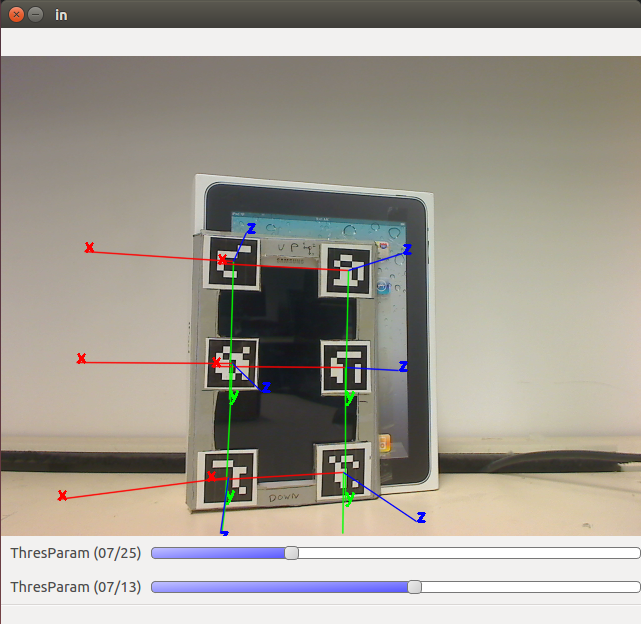
\includegraphics[scale=0.35]{images/output_aruco.png}
\caption{exemple of output of \texttt{ArUco} with 6 markers. Here the object-fixed reference frame $\{c\}$ is drawn}
\label{situation_validation}
\end{figure}

All methods give an estimate of $\mathbi{q}^c_a$ , that are compared with the data from the camera. The optical feedback provides a ground truth estimate for this experiment. To estimate the error that can occur with the optical feedback. We were careful in the experimentation to avoid the occlusion of the marker that is required to estimate the orientation. During this experiment, we applied a rotation of 90 degree around the $z_c$  on the smartphone in clockwise direction. Then, another rotation of 90 degree around the $z_c$ on the smartphone but in anticlockwise direction to return to the initial state. In order to study possible divergence of all methods. 


